\section{Results and Discussions}

This section presents the empirical results of our dual-pipeline system, comparing the
performance of the uncalibrated (No ArUco) model, which relies on scale-invariant depth ratios,
and the calibrated (ArUco) model, which resolves monocular scale ambiguity using physical
fiducial references. All evaluations are performed using a Group Shuffle Split (GSS) with a
$20\%$ test split grouped by mango ID, ensuring that validation and test metrics are computed
on completely unseen mango subjects.

\subsection{YOLOv11 Instance Segmentation Performance}
Prior to routing the feature vectors, the input RGB image is processed by the custom-trained
YOLOv11n instance segmentation model to isolate the mango fruit from the background. We
evaluated the performance of this segmentation stage on the validation split. The YOLOv11n-seg
model achieved exceptional performance, with box and mask precision of \textbf{99.9\%}, recall of
\textbf{100.0\%}, and mAP50 and mAP50-95 scores of \textbf{99.5\%}.

Table~\ref{tab:yolo_metrics} summarizes the performance metrics for both bounding boxes and
segmentation masks. The training loss curves are shown in Fig.~\ref{fig:yolo_training_results}.

\begin{table}[htbp]
\caption{YOLOv11n Instance Segmentation Performance}
\begin{center}
\begin{tabular}{|l|c|c|c|c|}
\hline
\textbf{Metric Group} & \textbf{Precision} & \textbf{Recall} & \textbf{mAP50} & \textbf{mAP50-95} \\
\hline
Bounding Box (Box) & 0.999 & 1.000 & 0.995 & 0.995 \\
Segmentation Mask (Mask) & 0.999 & 1.000 & 0.995 & 0.995 \\
\hline
\end{tabular}
\label{tab:yolo_metrics}
\end{center}
\end{table}

\begin{figure}[htbp]
    \centering
    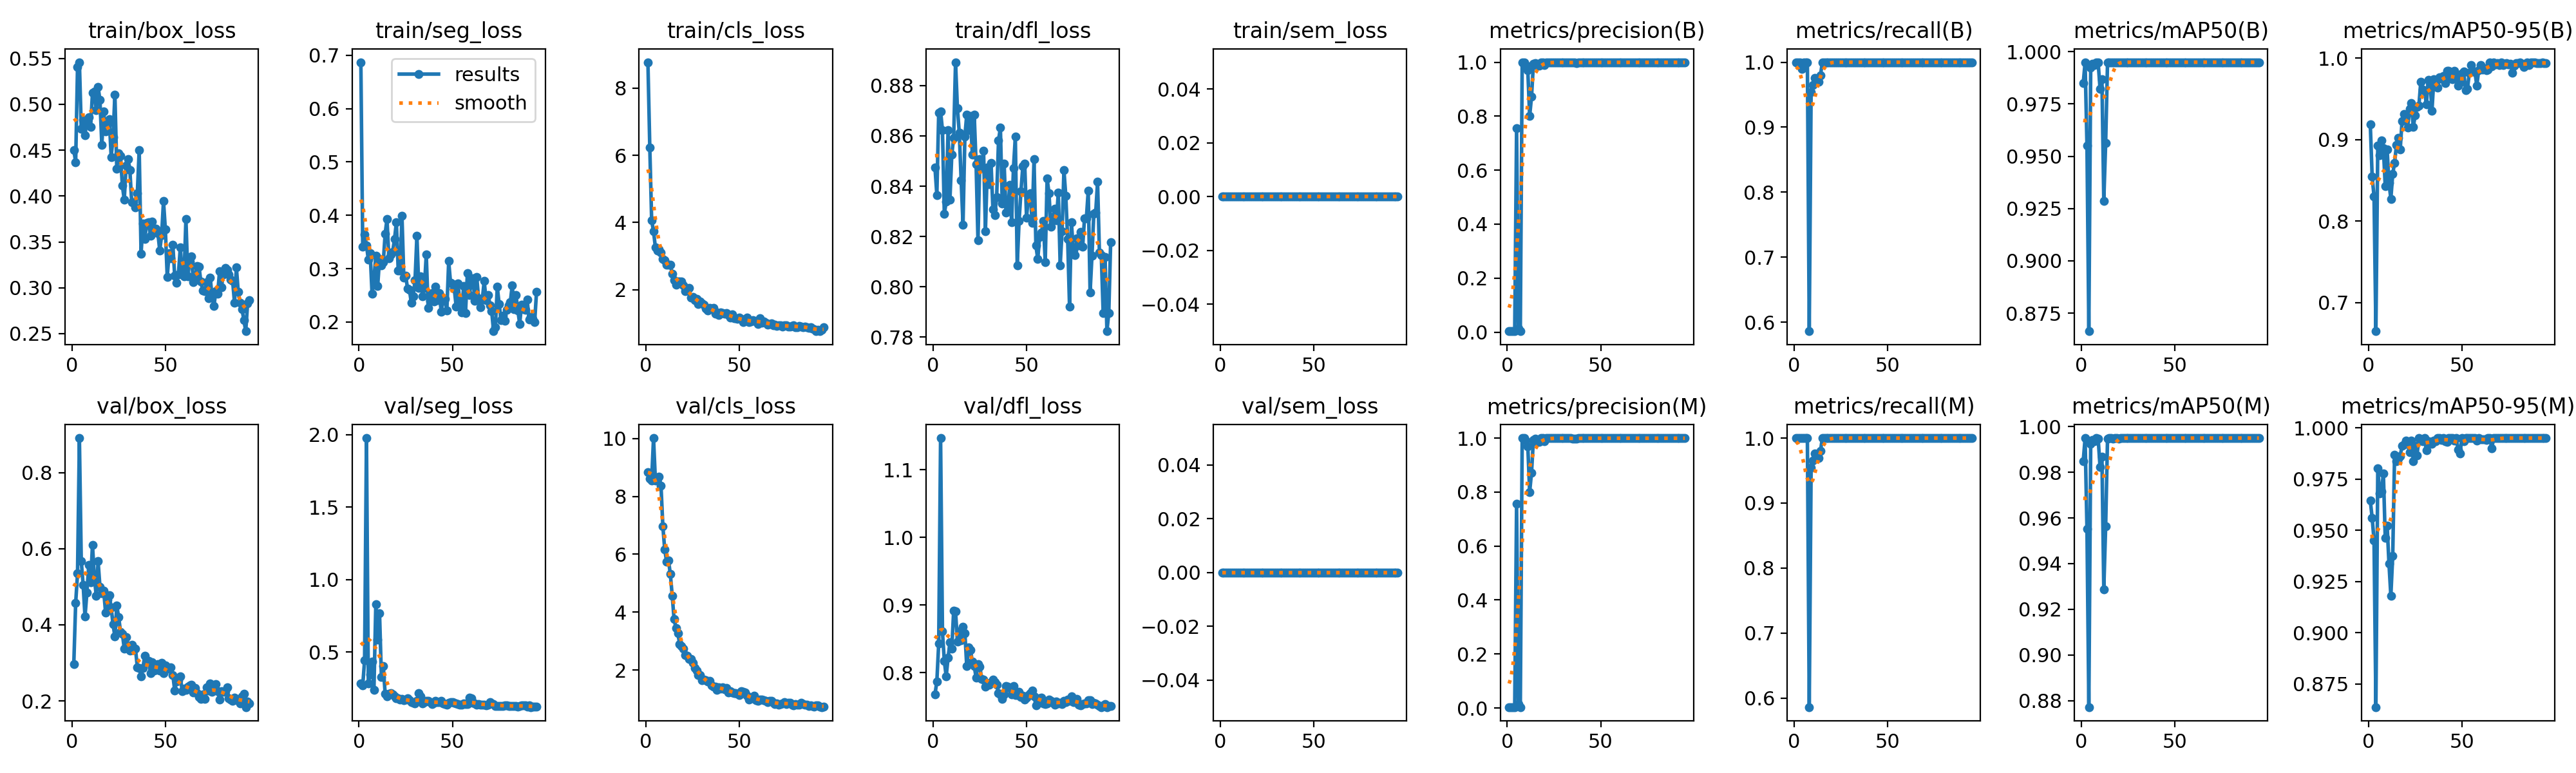
\includegraphics[width=0.85\columnwidth]{graphics/yolo_results.png}
    \caption{YOLOv11n-seg training metrics: training and validation loss curves (box, segment,
    class) and performance metrics (precision, recall, mAP) over 200 epochs.}
    \label{fig:yolo_training_results}
\end{figure}

These high metrics demonstrate that the custom-trained YOLOv11n-seg model forms an extremely
reliable frontend for our dual-pipeline architecture. By isolating the fruit boundary with near-
perfect accuracy, the model ensures that color, depth, and spatial features extracted in
subsequent stages are entirely free from background noise, even in challenging agricultural
setups with green foliage and varying lighting conditions.

\subsection{Orientation Classification Performance}
The Orientation Classification Model acts as a routing layer that automatically assigns the input mango image to one of five specialized orientation pipelines (Side, Top, Bottom, Front, or Back). A single, unified \textbf{MobileNetV3-Small} CNN — fine-tuned on the full 45-mango dataset (640 augmented images) — is shared by both the uncalibrated and ArUco-calibrated pipelines. Because orientation is determined purely from the RGB image crop and does not depend on depth calibration, a single model is sufficient for both pipelines.

Table~\ref{tab:orientation_metrics} summarizes the per-class performance of the CNN orientation classifier, and the corresponding confusion matrix is shown in Fig.~\ref{fig:orientation_cm}.

\begin{table}[htbp]
\caption{CNN Orientation Classification Performance (MobileNetV3-Small)}
\begin{center}
\begin{tabular}{|l|c|c|c|c|}
\hline
\textbf{Orientation} & \textbf{Precision} & \textbf{Recall} & \textbf{F1-Score} & \textbf{Support} \\
\hline
Back   & 1.00 & 0.90 & 0.95 & 21 \\
Bottom & 0.91 & 1.00 & 0.95 & 21 \\
Front  & 0.95 & 0.95 & 0.95 & 21 \\
Side   & 1.00 & 1.00 & 1.00 & 28 \\
Top    & 1.00 & 1.00 & 1.00 & 21 \\
\hline
\textbf{Overall} & \multicolumn{4}{c|}{\textbf{Accuracy: 97.32\%} (support = 112 images)} \\
\hline
\end{tabular}
\label{tab:orientation_metrics}
\end{center}
\end{table}

\begin{figure}[htbp]
    \centering
    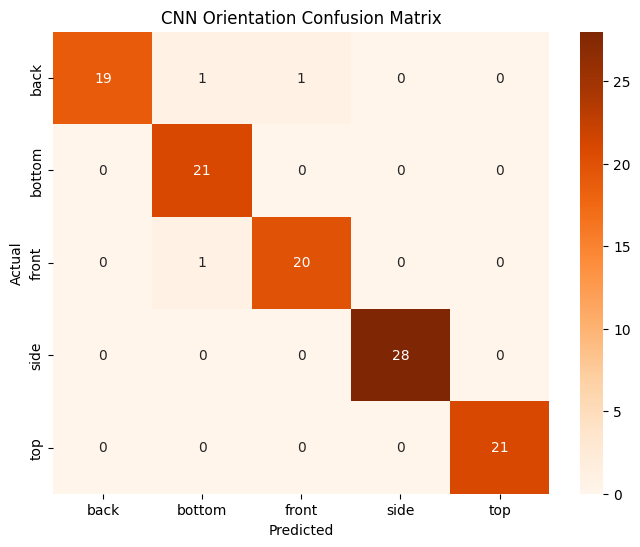
\includegraphics[width=0.85\columnwidth]{graphics/orientation_cm_cnn.png}
    \caption{Confusion matrix for the CNN Orientation Classification Model '(MobileNetV3-Small, 97.32\% accuracy).}
    \label{fig:orientation_cm}
\end{figure}

The unified CNN orientation model achieves an overall accuracy of \textbf{97.32\%} 
on 112 held-out test images from unseen mango subjects, representing a substantial improvement 
over the previous feature-based Random Forest classifiers (75.38\% uncalibrated, 62.50\% calibrated). 
The transfer-learning approach — fine-tuning a MobileNetV3-Small backbone pre-trained on 
ImageNet — allows the model to leverage rich visual features, almost completely eliminating 
inter-class confusion.

Per-class, the `top` and `side` views achieve perfect precision, recall, and F1-scores ($1.00$), 
as their distinct visual silhouettes (the circular stem-end profile of the top view and the elongated 
lateral profile of the side view) make them highly recognizable. The `back`, `bottom`, and `front` 
views also demonstrate robust classification with F1-scores of $0.95$. The minor remaining errors 
occur in the front/back/bottom transitions, where surface details can overlap under certain 
illumination conditions, though this confusion is greatly minimized compared to the baseline Random Forest classifiers.

\subsection{Ripeness Classification Performance}
The ripeness classification module evaluates the maturity stage of Katchamitha mangoes. 
Since Katchamitha mangoes exhibit green skin even when fully ripe, the models rely heavily 
on the CIELab color space coordinates ($a^*$ and $b^*$), which isolate subtle green-red and 
blue-yellow shifts. The classification results across all five views are shown in Table~\ref{tab:ripeness_results}.

\begin{table*}[htbp]
\caption{Ripeness Classification Accuracy Across Views}
\begin{center}
\begin{tabular}{|l|c|c|c|c|}
\hline
\textbf{View} & \multicolumn{2}{c|}{\textbf{Uncalibrated (No ArUco)}} & \multicolumn{2}{c|}{\textbf{Calibrated (ArUco)}} \\
\cline{2-5}
 & \textbf{Accuracy} & \textbf{F1 (Unripe / Ripe)} & \textbf{Accuracy} & \textbf{F1 (Unripe / Ripe)} \\
\hline
Side   & 71\% & 0.72 / 0.69 & 100\% & 1.00 / 1.00 \\
Top    & 89\% & 0.91 / 0.86 & 100\% & 1.00 / 1.00 \\
Bottom & 70\% & 0.75 / 0.64 & 100\% & 1.00 / 1.00 \\
Front  & 71\% & 0.67 / 0.75 & 100\% & 1.00 / 1.00 \\
Back   & 71\% & 0.50 / 0.80 & 100\% & 1.00 / 1.00 \\
\hline
\textbf{Overall} & \textbf{74.62\%} & \textbf{0.75 / 0.74} & \textbf{100.00\%} & \textbf{1.00 / 1.00} \\
\hline
\end{tabular}
\label{tab:ripeness_results}
\end{center}
\end{table*}

The uncalibrated ripeness classifiers show a robust performance, with accuracy ranging
from \textbf{70\%} (bottom) to \textbf{89\%} (top). The $a^*$ and $b^*$ color coordinates emerge
as the most important features in Gini importance charts, confirming that CIELab values
successfully capture the physiological shift in ripeness. 

The calibrated pipeline achieves a perfect \textbf{100\%} accuracy across all views. While this
suggests perfect classification, it represents an optimistic bound due to the limited size
of the ArUco dataset. With only 10 total mangoes, the GSS test set contains just 2 mangoes
(one ripe, one unripe). Because the test instances represent multiple augmented viewpoints
of the same two fruits, a correct classification on the individual fruit levels translates
to a $100\%$ score across all view subsets. This indicates that while the features are highly
discriminative, larger validation sets are required to confirm generalizability. The representative
confusion matrices for the side view ripeness classifier are shown in Fig.~\ref{fig:ripeness_cm}.

\begin{figure}[htbp]
    \centering
    \begin{tabular}{cc}
        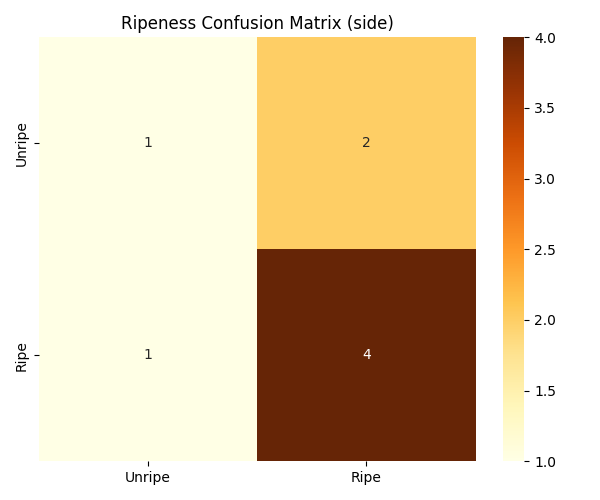
\includegraphics[width=0.45\columnwidth]{graphics/ripeness_cm_side_no_aruco.png} &
        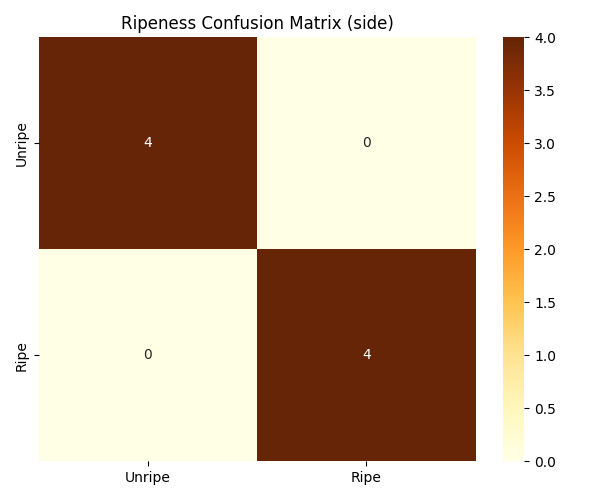
\includegraphics[width=0.45\columnwidth]{graphics/ripeness_cm_side_aruco.png} \\
        (a) Uncalibrated Pipeline & (b) Calibrated Pipeline
    \end{tabular}
    \caption{Confusion matrices for the Side View Ripeness Classifier.}
    \label{fig:ripeness_cm}
\end{figure}

\subsection{External Morphology Estimation}
The primary objective of Layer 1 regression models is to estimate the mango's physical
dimensions (height, width, thickness), volume, and weight. Table~\ref{tab:external_morphology}
compares the results of the two pipelines.

\begin{table*}[htbp]
\caption{Layer 1 External Morphology Performance Comparison ($R^2$ and MAE)}
\begin{center}
\begin{tabular}{|l|c|c|c|c|c|c|c|c|c|c|c|c|}
\hline
\textbf{View} & \multicolumn{4}{c|}{\textbf{Linear Dimensions (Height, Width, Thickness)}} & \multicolumn{4}{c|}{\textbf{Volumetric Group Space}} & \multicolumn{4}{c|}{\textbf{Gravimetric Mass Group}} \\
\cline{2-13}
 & \multicolumn{2}{c|}{\textbf{Uncalibrated}} & \multicolumn{2}{c|}{\textbf{Calibrated}} & \multicolumn{2}{c|}{\textbf{Uncalibrated}} & \multicolumn{2}{c|}{\textbf{Calibrated}} & \multicolumn{2}{c|}{\textbf{Uncalibrated}} & \multicolumn{2}{c|}{\textbf{Calibrated}} \\
\cline{2-13}
 & \textbf{$R^2$} & \textbf{MAE (cm)} & \textbf{$R^2$} & \textbf{MAE (cm)} & \textbf{$R^2$} & \textbf{MAE (cm$^3$)} & \textbf{$R^2$} & \textbf{MAE (cm$^3$)} & \textbf{$R^2$} & \textbf{MAE (g)} & \textbf{$R^2$} & \textbf{MAE (g)} \\
\hline
Side   & -0.1633 & 0.5225 & 0.4417 & 0.4228 & -0.0441 & 40.7241 & 0.8358 & 16.1094 & -0.0027 & 38.7450 & 0.8153 & 16.8236 \\
Top    &  0.0771 & 0.4929 & 0.5518 & 0.3361 &  0.2611 & 24.9339 & 0.6883 & 30.5792 &  0.3057 & 27.1427 & 0.7806 & 22.8484 \\
Bottom &  0.1755 & 0.5445 & 0.4084 & 0.4669 &  0.2335 & 30.4331 & 0.8522 & 16.7583 &  0.2367 & 35.6310 & 0.8243 & 18.6566 \\
Front  &  0.2363 & 0.5044 & 0.4660 & 0.4305 &  0.1781 & 36.8657 & 0.8718 & 15.1458 &  0.0267 & 37.0182 & 0.8405 & 18.2423 \\
Back   & -0.3062 & 0.5923 & 0.4809 & 0.4153 & -0.4748 & 42.1157 & 0.8752 & 13.7375 & -0.5543 & 46.2433 & 0.8643 & 14.9778 \\
\hline
\textbf{Overall} & \textbf{0.0039} & \textbf{0.5313} & \textbf{0.4698} & \textbf{0.4143} & \textbf{0.0308} & \textbf{35.0145} & \textbf{0.8247} & \textbf{18.4660} & \textbf{0.0024} & \textbf{36.9560} & \textbf{0.8250} & \textbf{18.3097} \\
\hline
\end{tabular}
\label{tab:external_morphology}
\end{center}
\end{table*}

The comparison reveals a stark difference between the two architectures:
\begin{enumerate}
    \item \textbf{Uncalibrated Pipeline Failure:} The uncalibrated models yield very poor
    morphological estimations, with $R^2$ values frequently falling below zero (e.g., Side
    view Volumetric $R^2 = -0.04$, Gravimetric $R^2 = -0.00$; Back view Volumetric $R^2 = -0.47$,
    Gravimetric $R^2 = -0.55$). Negative $R^2$ scores indicate that the model performs worse
    than a simple horizontal line predicting the dataset mean. This occurs due to the
    \textit{scale ambiguity} of monocular depth estimation. Without an absolute reference,
    depth maps provide only relative depths. Consequently, the relationship between features in
    raw pixel values and their corresponding physical units is highly unstable, preventing the
    regression model from generalizing.
    \item \textbf{Calibrated Pipeline Success:} Incorporating the ArUco marker to calibrate
    the depth scale resolves the scale ambiguity. The calibrated models achieve high estimation
    accuracy. Volumetric and Gravimetric regression achieve $R^2$ values of \textbf{0.78--0.87},
    with Mean Absolute Errors (MAE) reduced to \textbf{13.7--30.5 cm$^3$} for volume and
    \textbf{14.9--22.8 grams} for weight (mass). The linear dimensions regression (height, width,
    thickness) also shows a major improvement, achieving $R^2$ scores of \textbf{0.40--0.55}
    and MAEs below \textbf{0.47 cm}.
\end{enumerate}

These findings demonstrate that while monocular depth maps are highly useful for capturing
3D shape contours, absolute metric calibration using physical fiducial markers is essential
to achieve acceptable accuracy for sorting and grading tasks.

\subsection{Layer 2 Internal Seed Morphology Estimation}
Layer 2 regresses the dimensions, volume, and weight of the internal mango bone (seed/endocarp) based on the estimated external properties (dimensions, volume, weight) and ripeness from Layer 1. The results are summarized in Table~\ref{tab:internal_morphology}.

\begin{table*}[htbp]
\caption{Layer 2 Internal Seed Morphology Results ($R^2$ and MAE)}
\begin{center}
\begin{tabular}{|l|c|c|c|c|}
\hline
\textbf{Semantic} & \multicolumn{2}{c|}{\textbf{Uncalibrated (No ArUco)}} & \multicolumn{2}{c|}{\textbf{Calibrated (ArUco)}} \\
\cline{2-5}
\textbf{Group (Seed)} & \textbf{$R^2$} & \textbf{MAE} & \textbf{$R^2$} & \textbf{MAE} \\
\hline
Linear Dimensions & 0.6193 & 0.1689 cm & 0.5999 & 0.1820 cm \\
Volumetric Space  & 0.8452 & 2.3405 cm$^3$ & 0.9417 & 1.8000 cm$^3$ \\
Gravimetric Mass  & 0.8437 & 1.9884 grams & 0.9077 & 1.9187 grams \\
\hline
\end{tabular}
\label{tab:internal_morphology}
\end{center}
\end{table*}

Both pipelines achieve high performance for predicting internal seed properties. The
uncalibrated Layer 2 model yields $R^2$ scores of \textbf{0.84} for volume and weight,
and the calibrated model yields $R^2$ scores of \textbf{0.90--0.94} for volume and
weight. 

This high performance is driven by the \textbf{allometric scaling relationships} inherent
in biological fruits: the internal endocarp's volume and weight scale predictably with
the overall size and mass of the external fruit. Since Layer 2 takes external properties
(which are highly accurate in the calibrated case, or ground-truth values during training)
and ripeness as inputs, the Random Forest model is able to learn the physical mapping
and predict internal seed traits with high precision. This is particularly valuable as it
enables the non-destructive estimation of the stone-to-flesh ratio, which is historically
difficult to estimate without physical cut-testing. Feature importance charts (Fig.~\ref{fig:seed_fi})
show that the external weight and volume are the most influential inputs for mapping
the seed dimensions, confirming the biological basis of the model.

\begin{figure}[htbp]
    \centering
    \begin{tabular}{cc}
        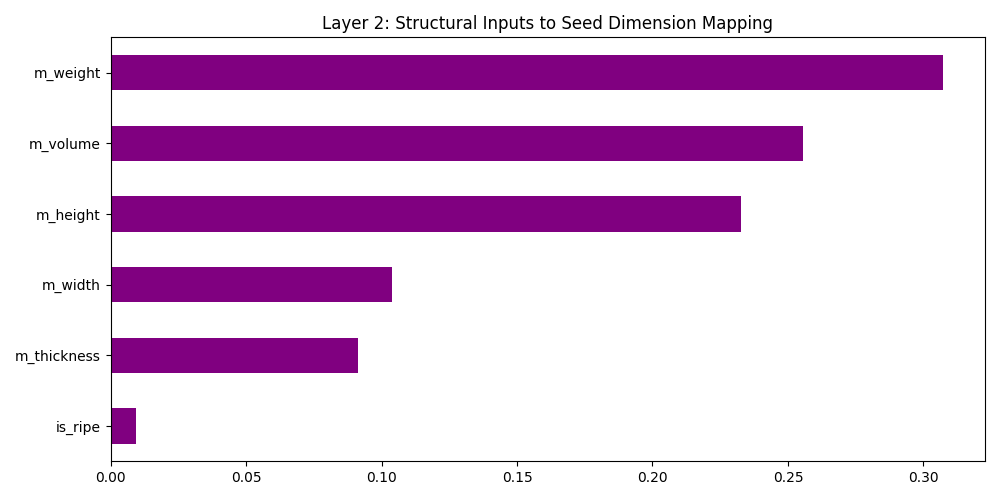
\includegraphics[width=0.45\columnwidth]{graphics/seed_fi_no_aruco.png} &
        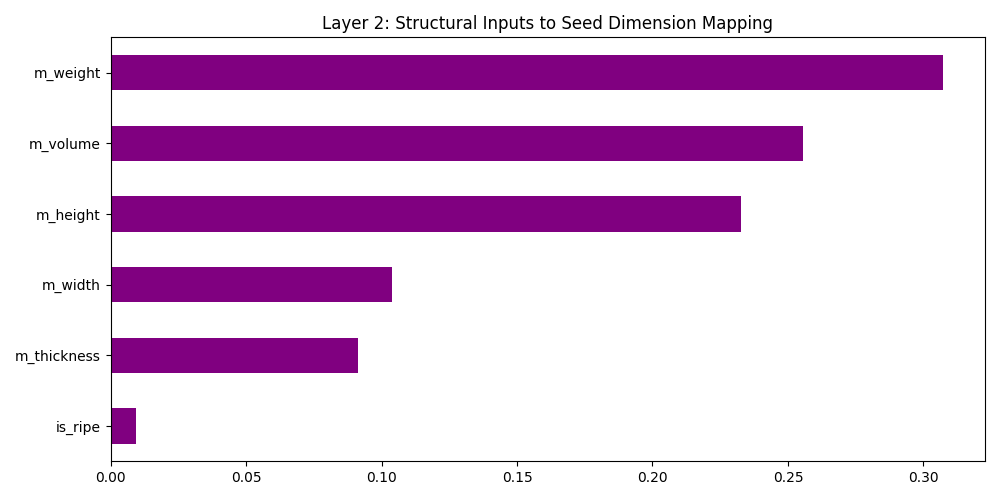
\includegraphics[width=0.45\columnwidth]{graphics/seed_fi_aruco.png} \\
        (a) Uncalibrated Pipeline & (b) Calibrated Pipeline
    \end{tabular}
    \caption{Feature importance charts for the Layer 2 Internal Seed Regressor.}
    \label{fig:seed_fi}
\end{figure}
